%% manuscript/main.tex
%% SAI / IJACSA paper format (IEEEtran conference class from thesai.org ZipFileHandler).
\documentclass[conference, letterpaper]{IEEEtran}

\usepackage[pdftex]{graphicx}
\usepackage[cmex10]{amsmath}
\usepackage{amssymb}
\usepackage{booktabs}
\usepackage{cite}
\usepackage{url}
\usepackage{hyperref}
\usepackage{fancyhdr}
\usepackage{balance}
\usepackage{xcolor}

\hypersetup{
  colorlinks=true,
  linkcolor=black,
  citecolor=black,
  urlcolor=black,
  pdfauthor={},
  pdftitle={Partition Draws, Not Aggregators: Decomposing Result Variance in Federated LoRA Fine-Tuning Under Non-IID Splits}
}

\graphicspath{{../figures/}{figures/}}

% SAI header/footer (from Paper_format.tex)
\pagestyle{fancy}
\fancyhf{}
\fancyhead[L]{\footnotesize International Journal of Advanced Computer Science and Applications,}
\fancyhead[R]{\footnotesize Vol.\ , No.\ , 2026}
\renewcommand{\headrulewidth}{0.5pt}
\fancyfoot[C]{www.ijacsa.thesai.org}
\renewcommand{\footrulewidth}{0.5pt}
\fancyfoot[R]{\thepage \  $|$ P a g e }

\begin{document}

\title{Partition Draws, Not Aggregators: Decomposing Result Variance in Federated LoRA Fine-Tuning Under Non-IID Splits}

% Author block retained for assembly; anonymized in Phase M step 4.
\author{\IEEEauthorblockN{Jerry Adams Franklin}
\IEEEauthorblockA{Independent Researcher\\
Email: jerryadamsfranklin@example.com}
}

\maketitle

\begin{abstract}
Federated LoRA comparisons often rest on a single non-IID partition draw, even when reported method gaps sit near ordinary run-to-run noise. We ask how much of the variation in held-out next-token loss comes from the partition draw, how often few-draw rankings flip, and how many draws a target effect size requires. In a pre-registered design of $120$ runs at two scales (TinyLlama-1.1B-Chat and LLaMA-3.2-3B), with partition seeds separated from training seeds, we fit a two-way variance decomposition for FedIT, FFA-LoRA, and FLoRA on Dolly, partitioned by its category labels at Dirichlet $\alpha{=}0.1$. On TinyLlama the partition and interaction shares are $0.508$ and $0.469$ against a residual of $0.023$. On LLaMA-3.2-3B the interaction dominates ($0.764$) and the partition interval includes zero. Ranking flips concentrate in the near-tied FedIT--FLoRA pair: the three-draw paired flip probability is $0.377$, while gaps of about $0.023$ never reverse in a single draw. Detecting that observed near-tie at $80\%$ power needs $206$ paired partition draws on TinyLlama and $46$ on LLaMA-3.2-3B; separable pairs need only $3$. We recommend reporting the number of partition draws, pairing comparisons on partitions, and stating the smallest difference the design can detect. We make no method recommendation.
\end{abstract}

\begin{IEEEkeywords}
federated learning; low-rank adaptation; non-IID partitioning; experimental variance; reproducibility; large language models
\end{IEEEkeywords}


\IEEEpeerreviewmaketitle

\section{Introduction}
\label{sec:intro}

Federated LoRA methods for instruction tuning report method differences that are often small relative to the noise in a single evaluation. FFA-LoRA~\cite{sun2024ffalora} publishes means over $20$ runs with standard deviations; in the non-private setting the LoRA standard deviation on MNLI-matched ($10.7$) exceeds the mean gap to FFA-LoRA ($3.02$ points). FLoRA~\cite{wang2024flora} compares to FedIT~\cite{zhang2024fedit} with single reported MMLU and MT-bench values after $1$ to $3$ communication rounds, without reported seed replication, including a Llama/Alpaca MMLU margin of $0.44$ points that the paper itself calls ``marginal.'' Those practices establish the motivating fact: published federated LoRA contrasts can sit inside, or only slightly above, ordinary run-to-run variation. What they do not establish is how much of that variation comes from the non-IID partition draw itself.

In Dirichlet or category-based federated simulations, the ``non-IID'' condition is commonly instantiated from a single partition seed: the Dirichlet construction itself~\cite{hsu2019measuring} and the partition catalogues built on it~\cite{li2022niidbench} treat the draw as a setting rather than a source of variance. In the evaluations cited above, training seeds are sometimes repeated while the partition seed is not. If held-out loss moves with the partition draw by as much as it moves with the training seed, then a ranking obtained from one or two partitions is not a property of the methods alone. The open question is quantitative: how large is the partition component, how often do few-draw rankings flip, and how many draws are needed for a target effect size?

We answer three pre-registered questions on FedIT, FFA-LoRA, and FLoRA, using held-out next-token loss on Dolly as the response. All differences are in held-out next-token loss, where the unadapted base models score $2.121$ and $2.169$ and fine-tuned runs fall between $1.69$ and $1.841$. The design freezes the federation (ten clients, full participation, fifteen rounds, one local epoch), the LoRA configuration, and the analysis plan before any production run, and separates partition seeds from training seeds at two model scales.

\begin{itemize}
\item \textbf{RQ1.} At Dirichlet $\alpha{=}0.1$, what share of the variance comes from the partition draw, the partition-by-method interaction, and the training seed?
\item \textbf{RQ2.} How often does an evaluation using $k$ partition draws rank the three methods differently from the full-design ranking?
\item \textbf{RQ3.} How many partition draws are needed to detect held-out loss differences of $0.005$, $0.01$, $0.02$, and $0.05$ at $80\%$ power, for paired and unpaired designs?
\end{itemize}

An exploratory RQ4 on partition statistics is reported but not used for claims.

\paragraph{Advance over the state of the art.}
Prior federated LoRA evaluations either report multi-seed means without separating the partition draw from the training seed, or treat the non-IID split as a fixed setting rather than a variance component. Adjacent work decomposes variance over training or unlearning seeds and over benchmark variants, but not over the federated partition draw for LoRA instruction tuning. This paper's advance is to isolate that draw in a pre-registered design, quantify its share relative to interaction and residual noise, and turn the measurement into an explicit reporting protocol that states how many draws were used, that comparisons were paired on those draws, and what minimum difference the design can detect. The same design also shows the cost of too few draws: extending LLaMA-3.2-3B from six to ten partitions reverses the FedIT--FLoRA top-two order and grows the interaction component by a factor of $2.66$.

\paragraph{Contributions.}
(1)~A pre-registered $120$-run design at two scales (TinyLlama-1.1B-Chat and LLaMA-3.2-3B), extended by $84$ further runs, that separates partition seeds from training seeds under a frozen federation and LoRA configuration. (2)~A method-of-moments variance decomposition with cluster-bootstrap intervals, showing on TinyLlama that partition and interaction shares dominate the residual ($0.508$ and $0.469$ versus $0.023$), while on LLaMA-3.2-3B at $p{=}10$ the interaction dominates ($0.992$) and the partition main-effect interval includes zero after truncation. (3)~A ranking-stability analysis conditioned on effect size: the near-tied FedIT--FLoRA pair flips under few draws (three-draw paired flip probability $0.377$ on TinyLlama and $0.493$ on LLaMA-3.2-3B), whereas gaps of about $0.023$ to $0.031$ never reverse in a single draw. (4)~A draws-needed table for pre-registered deltas and for the observed gaps, including $206$ and more than $1000$ paired draws for the near-tie at the two scales, and the observation that where the interaction dominates, pairing on partitions buys little. (5)~The Partition-Draw Reporting Protocol as three numbered steps (partition-draw count and seeds; paired comparisons; detectable minimum difference). We make no method recommendation.

Section~\ref{sec:related} situates the work against benchmark-variance studies, non-IID simulation practice, and federated LoRA evaluation. Section~\ref{sec:setup} states the design and variance model. Section~\ref{sec:results} reports the measurements. Section~\ref{sec:discussion} gives reporting recommendations and limitations. Section~\ref{sec:conclusion} concludes.

\section{Related Work}
\label{sec:related}

\paragraph{Variance and seed sensitivity in ML benchmarks.}
Empirical comparisons are sensitive to sources of variation beyond the method under test. Bouthillier et al.~\cite{bouthillier2021accounting} model data sampling, initialization, and hyperparameter choice as variance components in machine-learning benchmarks and show that ignoring them inflates the chance of declaring a false improvement; their recommendations include randomizing multiple sources of variation and accounting for the resulting uncertainty when claiming gains. Picard~\cite{picard2021seed} isolates the random seed alone: across $10{,}000$ CIFAR-10 trainings the accuracy range reached $1.82$ percentage points, and a smaller but still material range appeared on ImageNet. Both lines of work motivate multi-seed summaries and caution around small margins. Neither separates the draw of a federated data partition from the training seed, which is the decomposition this paper targets.

\paragraph{Non-IID simulation in federated learning.}
Federated evaluations routinely induce client heterogeneity by construction. Hsu et al.~\cite{hsu2019measuring} synthesize label skew by drawing each client's class proportions from a Dirichlet distribution $\mathrm{Dir}(\alpha p)$, with smaller $\alpha$ producing more skewed clients, and show FedAvg accuracy falling as identicalness decreases (for example, improving a highly skewed CIFAR-10 setting from $30.1\%$ to $76.9\%$ with server momentum). Natural partitions that follow writers, users, or categories appear in benchmarks such as LEAF~\cite{caldas2019leaf}. Federated instruction-tuning papers inherit both practices: FedIT~\cite{zhang2024fedit} assigns Dolly categories to clients under a synthetic shard, and FFA-LoRA~\cite{sun2024ffalora} uses fixed heterogeneous label splits rather than a Dirichlet draw. What is rarely varied is the partition seed itself; a single draw is treated as the non-IID condition, even when that draw determines which clients are empty of a category or too small to take an optimizer step.

\paragraph{Federated LoRA methods and evaluation practice.}
FedIT~\cite{zhang2024fedit} aggregates LoRA adapters with FedAvg for instruction tuning. FFA-LoRA~\cite{sun2024ffalora} freezes $A$ and trains $B$, reporting accuracy over $20$ runs with mean and standard deviation; even in the non-private setting, method gaps can be small (for example, $85.05$ versus $82.03$ on MNLI-matched, and $84.35$ versus $83.51$ on QNLI). FLoRA~\cite{wang2024flora} stacks heterogeneous-rank adapters and compares to FedIT on MMLU and MT-bench; several margins are likewise modest (Llama/Alpaca MMLU $29.85$ versus $29.41$; the paper itself calls the Alpaca gap ``marginal,'' and homogeneous MT-bench gains are described as at least $0.2$). Published evaluations therefore often report multi-seed means, yet they do not resample the partition draw, nor do they test whether rankings survive that resampling when the reported margin is on the order of a point or less.

\paragraph{Gap.}
No prior study decomposes partition-draw variance against training-seed variance for federated LoRA instruction tuning, or tests whether method rankings survive that partition variance. This paper fills that gap under a pre-registered design.

\section{Experimental Setup}
\label{sec:setup}

We study three federated LoRA aggregation methods that appear in recent instruction-tuning work: FedIT (FedAvg over LoRA adapters), FFA-LoRA, and FLoRA. No other aggregators are included. The design is fixed before production runs and is identical across methods except for the aggregation rule itself.

\paragraph{Models and adapters.}
The primary model is TinyLlama-1.1B-Chat-v1.0. The replication model is LLaMA-3.2-3B, retained after a timing gate on an RTX 4090 showed a median production wall-clock of about 51 minutes per run and a peak allocation near 9~GB. Both models use the same LoRA configuration: rank $r{=}16$, scaling $\alpha_{\mathrm{LoRA}}{=}32$, dropout $0.1$, and target modules restricted to \texttt{q\_proj} and \texttt{v\_proj}. The base model is frozen; only the LoRA parameters are trained and communicated.

\paragraph{Federation.}
Each run uses 10 clients with full participation for 15 rounds and one local epoch per round. TinyLlama uses batch size 4 with gradient accumulation 4; LLaMA-3.2-3B uses batch size 2 with gradient accumulation 8. Learning rate, sequence length (256), and weight decay follow the frozen configuration files. The client training loop steps the optimizer only on complete gradient-accumulation blocks and does not use \texttt{drop\_last}. Clients whose local set is smaller than one full block therefore contribute zero optimizer steps and upload the unchanged global adapter. Under the TinyLlama loader, that threshold is at most 12 samples; under the LLaMA loader it is at most 14. In the Dirichlet $\alpha{=}0.1$ partitions, zero-step clients hold at most 11 samples, effective clients (those with at least one step) range from 7 to 10 on TinyLlama, and discarded trailing samples per partition seed range from 27 to 60 on TinyLlama and from 41 to 104 on LLaMA-3.2-3B. Client sizes in those partitions range from 2 to 1218.

\paragraph{Data and partitions.}
All training examples come from Databricks Dolly-15k, using \texttt{train}$[0{:}3000]$. The non-IID setting is Dirichlet label skew over the dataset's real \texttt{category} column at $\alpha{=}0.1$. The IID setting uses a single fixed data seed. Partition draws are controlled by data seeds that are separate from the training (run) seeds. TinyLlama uses data seeds 2001--2010 with run seeds $\{7001,7002\}$ at $\alpha{=}0.1$ (60 cells) and data seed 2001 with run seeds 7001--7005 for IID (15 cells). LLaMA-3.2-3B uses data seeds 2001--2006 with the same two run seeds at $\alpha{=}0.1$ (36 cells) and data seed 2001 with run seeds 7001--7003 for IID (9 cells). The total design is 120 production cells. Active clients under $\alpha{=}0.1$ take only the values 9 or 10.

\paragraph{Held-out metric.}
The primary metric is held-out next-token loss on Dolly \texttt{train}$[3000{:}3500]$ (500 examples), maximum sequence length 256, using the same prompt format as training, including a \texttt{Context} field when present (formatter version \texttt{v2-dolly-context}). Base (unadapted) held-out loss is 2.120666 on TinyLlama and 2.168946 on LLaMA-3.2-3B and is constant within each model to machine precision across runs. TinyLlama holdout evaluation runs in float32. LLaMA-3.2-3B production holdouts run in float16 with sequential loading (the tuned adapter is freed before the base model is loaded) because two concurrent float32 3B copies exceed 24~GB. A float32 spot-check on three LLaMA cells spanning the production tuned-loss range found a maximum absolute difference of $4.1{\times}10^{-5}$ relative to float16, about 250 times below the 0.01 effect scale used for power calculations, so float16 was retained for the LLaMA production numbers.

\paragraph{Communication.}
Secondary reporting uses measured communication in megabytes. Per-client upload payloads match the frozen constants: 9{,}011{,}200 bytes for TinyLlama (FedIT and FLoRA) and 9{,}175{,}040 bytes for LLaMA-3.2-3B (FedIT and FLoRA). FFA-LoRA, as implemented in this codebase, uploads both $A$ and $B$ on the first round and $B$ thereafter, and downloads $B$ only (3{,}244{,}032 bytes per client on TinyLlama). Total communication therefore differs across methods by construction. We report communication only within method across partitions and do not rank methods by bytes.

\paragraph{Hardware and software provenance.}
Every production cell ran on a single NVIDIA GeForce RTX 4090 with one worker process per GPU. Median wall-clock time is 27.1 minutes for TinyLlama and 51.1 minutes for LLaMA-3.2-3B. Training provenance is the \texttt{freeze-v1} tag with a clean tracked tree. The LLaMA float16 holdout change is an eval-only amendment tagged \texttt{freeze-v2}; it does not alter training code or aggregated adapters. Three cells resumed from a checkpoint after host hangs (one TinyLlama FLoRA cell and two LLaMA FLoRA cells); their held-out losses fall inside the range of the other run seeds that share the same grid, heterogeneity, data seed, and method.


\begin{table}[!t]
\centering
\caption{Frozen experimental design.}
\label{tab:setup}
\small
\begin{tabular}{ll}
\toprule
Element & Value \\
\midrule
Methods & FedIT, FFA-LoRA, FLoRA \\
Models & TinyLlama-1.1B-Chat-v1.0; LLaMA-3.2-3B \\
LoRA & $r{=}16$, $\alpha{=}32$, dropout $0.1$, $q\_proj$+$v\_proj$ \\
Federation & 10 clients, full participation, 15 rounds, 1 local epoch \\
Data & Dolly-15k train$[0{:}3000]$; held-out train$[3000{:}3500]$ \\
Non-IID & Dirichlet label skew on \texttt{category}, $\alpha{=}0.1$ \\
IID & Fixed data seed split \\
Primary metric & Held-out loss (formatter \texttt{v2-dolly-context}) \\
Secondary & Measured communication (MB) \\
TinyLlama cells & 60 ($\alpha{=}0.1$) + 15 (IID) \\
LLaMA-3.2-3B cells & 36 ($\alpha{=}0.1$) + 9 (IID) \\
\bottomrule
\end{tabular}

\end{table}

\section{Results}
\label{sec:results}

All analyses use held-out loss as the response. Numbers below come from the pre-registered tables in \texttt{analysis/}. We report TinyLlama and LLaMA-3.2-3B separately and do not recommend a method.

\paragraph{Variance components at $\alpha{=}0.1$.}
Table~\ref{tab:variance} summarizes the method-of-moments estimates under the two-way design in Section~\ref{sec:setup}. On TinyLlama ($p{=}10$), the partition share is $\hat\sigma^2_P/(\hat\sigma^2_P{+}\hat\sigma^2_{PM}{+}\hat\sigma^2_E){=}0.508$ with bootstrap 95\% CI $[0.202,0.663]$, the interaction share is $0.469$ $[0.316,0.765]$, and the residual share is $0.023$ $[0.007,0.056]$. Absolute components are $\hat\sigma^2_P{=}4.09{\times}10^{-6}$, $\hat\sigma^2_{PM}{=}3.78{\times}10^{-6}$, and $\hat\sigma^2_E{=}1.89{\times}10^{-7}$. Partition and interaction are comparable in magnitude; residual training-seed noise is an order of magnitude smaller. No estimate was truncated at zero. The pre-registered mixed-model cross-check recovers the residual component on both models ($1.89{\times}10^{-7}$ and $1.31{\times}10^{-7}$, matching $\hat\sigma^2_E$) and a method-level variance component comparable to $\hat\sigma^2_P{+}\hat\sigma^2_{PM}$, but the separate partition component did not identify under the specified variance-component formula. We therefore report the moment estimates as primary, as pre-registered, and treat the mixed model as a partial cross-check.

On LLaMA-3.2-3B ($p{=}6$), the interaction dominates: share $0.764$ $[0.443,0.990]$, with $\hat\sigma^2_{PM}{=}1.11{\times}10^{-5}$. The partition share is $0.227$ $[0.000,0.551]$ and the residual share is $0.009$ $[0.002,0.043]$, with $\hat\sigma^2_P{=}3.28{\times}10^{-6}$ and $\hat\sigma^2_E{=}1.31{\times}10^{-7}$. Because the partition CI includes zero, we do not claim a partition main effect at 3B; the 3B story is the interaction. Cross-scale bootstrap CIs on the partition share overlap ($[0.202,0.663]$ versus $[0.000,0.551]$), so the data do not distinguish the two scales on that margin. No estimate was truncated at zero.

\paragraph{IID noise floor.}
Pooling the per-method IID variances gives $6.40{\times}10^{-8}$ on TinyLlama and $3.07{\times}10^{-7}$ on LLaMA-3.2-3B. The ratio of $\hat\sigma^2_E$ at $\alpha{=}0.1$ to this IID floor is $2.96$ on TinyLlama. On LLaMA the ratio is $0.43$, but each method's IID variance has only two degrees of freedom (three run seeds), and the per-method IID variances differ by more than an order of magnitude ($2.4{\times}10^{-8}$ for FFA-LoRA versus $6.6{\times}10^{-7}$ for FLoRA). We therefore report the 3B IID floor descriptively and do not interpret the ratio below one as evidence that $\alpha{=}0.1$ is quieter than IID.

\paragraph{Ranking stability.}
The reference ranking at $\alpha{=}0.1$ orders methods by mean held-out loss over all cells: TinyLlama ranks FLoRA, FedIT, then FFA-LoRA; LLaMA ranks FedIT, FLoRA, then FFA-LoRA. Under the pre-registered paired protocol ($B{=}10{,}000$), the probability that the best method differs from this reference equals the probability that the full order differs (the two coincide because the only pair whose order changes is the top one; the third method is separated by an order of magnitude more than the per-draw noise). On TinyLlama those probabilities are $0.555$, $0.406$, $0.377$, and $0.284$ for $k{\in}\{1,2,3,5\}$ (Wilson 95\% CI half-widths about $0.01$). On LLaMA they are $0.168$, $0.272$, and $0.287$ for $k{\in}\{1,2,3\}$. Unpaired probabilities are similar in magnitude and are shown in Figure~\ref{fig:flip} and \texttt{analysis/rank\_flip.csv}; the paired protocol is primary.

The aggregate flip rate is entirely the near-tied FedIT--FLoRA pair. On TinyLlama that pair has true mean gap $+0.00055$; single-draw sign flips occur in 11 of 20 cells, and the paired order-flip probability is $0.555$ at $k{=}1$ and $0.377$ at $k{=}3$. The separable pairs (FedIT versus FFA-LoRA at $-0.023$, FFA-LoRA versus FLoRA at $+0.024$) never reverse: 0 of 20 single draws and paired flip probability $0$ at every $k$. On LLaMA, FedIT versus FLoRA has gap $-0.0020$ with 2 of 12 single-draw sign flips and paired flip probabilities $0.168$ ($k{=}1$) and $0.287$ ($k{=}3$); the separable gaps $-0.033$ (FedIT versus FFA-LoRA) and $+0.031$ (FFA-LoRA versus FLoRA) never flip (0 of 12). The rise in LLaMA flip probability from $k{=}1$ to $k{=}3$ is a small-sample artifact of six partitions and a near-tie, not evidence that more draws are worse.

Conditioned on effect size, the ranking claim is therefore: pairs separated by less than the per-draw paired SD ($0.00282$ on TinyLlama, $0.00473$ on LLaMA; empirical means $0.00276$ and $0.00461$) are ordered near-randomly by a few-partition evaluation, while gaps of about $0.023$ (TinyLlama) and $0.031$ (LLaMA) were recovered in every single draw. The flip table is a restatement of that conditioning, not a separate claim about method quality.

\paragraph{Draws needed.}
Using the model-based paired SD, detecting a pre-registered $\Delta{=}0.005$ at 80\% power (two-sided $\alpha{=}0.05$) requires $5$ paired partition draws on TinyLlama and $10$ on LLaMA; $\Delta{=}0.01$ requires $3$ and $5$; $\Delta{=}0.02$ requires $3$ and $3$; $\Delta{=}0.05$ requires $2$ and $3$. Unpaired per-method $n$ values are similar (TinyLlama $7$, $3$, $2$, $2$; LLaMA $11$, $4$, $3$, $2$). For the observed gaps, the near-tie would need $206$ paired draws on TinyLlama and $46$ on LLaMA, whereas each separable pair needs only $3$ paired draws on either model. That contrast is the operational form of the ranking result: a few partitions suffice when the gap is large relative to the paired SD, and hundreds are required when it is not.

\paragraph{Observed method differences.}
Table~\ref{tab:means} reports means and SDs. At $\alpha{=}0.1$, TinyLlama means are FLoRA $1.6957$ (SD $0.0013$), FedIT $1.6962$ ($0.0038$), and FFA-LoRA $1.7192$ ($0.0026$), each over $n{=}20$ cells; LLaMA means are FedIT $1.8028$ ($0.0051$), FLoRA $1.8049$ ($0.0020$), and FFA-LoRA $1.8355$ ($0.0031$), each over $n{=}12$. Paired $t$-tests on partition-level means with Holm correction~\cite{dror2018hitchhiker} reject FFA-LoRA versus each of the other two methods on both models (TinyLlama Holm $p{<}10^{-8}$; LLaMA Holm $p{<}10^{-4}$) and do not reject FedIT versus FLoRA (TinyLlama Holm $p{=}0.57$; LLaMA Holm $p{=}0.41$). The FedIT--FLoRA confidence intervals include zero on both models. We report these contrasts as context for the ranking and power sections and do not claim a winning method.

\paragraph{Partition statistics and communication.}
Among five exploratory Spearman correlations of partition-mean held-out loss with partition statistics, TinyLlama mean Jensen--Shannon divergence has $\rho{=}0.72$ ($p{=}0.019$, $n{=}10$). That association does not survive Holm correction across the five TinyLlama tests (Holm $p{=}0.093$) and does not replicate on LLaMA ($\rho{=}0.086$, $p{=}0.87$, $n{=}6$). Active clients vary only from 9 to 10 and show no reliable association ($\rho{=}0.35$, $p{=}0.32$ on TinyLlama; $\rho{=}0.13$, $p{=}0.80$ on LLaMA). We treat RQ4 as exploratory and do not build an argument on any single correlation.

Measured total communication matches the V6 payload formula exactly for all six method--model pairs ($\max|\mathrm{error}|{=}0$). Across $\alpha{=}0.1$ partitions, TinyLlama totals range from $2320.3$ to $2578.1$~MB for FedIT and FLoRA and from $884.8$ to $983.1$~MB for FFA-LoRA; LLaMA ranges are $2362.5$ to $2625.0$~MB and $992.3$ to $1102.5$~MB. The FFA-LoRA range is lower because this implementation transmits $A$ and $B$ only in the first round and $B$ alone thereafter, in both directions; we report the values as measured within method and do not rank methods by bytes.

\paragraph{Pre-registered claim mapping.}
Following the outcome-to-claim table, TinyLlama triggers row~1 on the partition share ($0.508$). LLaMA triggers row~1 only through the three-draw flip probability ($0.287$), with the near-tie caveat above, and additionally triggers row~4 because the interaction share ($0.764$) exceeds the partition share. Cross-scale partition-share CIs overlap (row~6). No other pre-registered claim rows are selected for either model.


\begin{table*}[!t]
\centering
\caption{Method-of-moments variance components at Dirichlet $\alpha{=}0.1$ with bootstrap 95\% CIs over partitions ($B{=}2000$).}
\label{tab:variance}
\small
\begin{tabular}{llrrrlllrrr}
\toprule
Model & Setting & $\hat\sigma^2_P$ & $\hat\sigma^2_{PM}$ & $\hat\sigma^2_E$ & Share $P$ & Share $PM$ & Share $E$ & $p$ & $m$ & $r$ \\
\midrule
TinyLlama-1.1B & $\alpha{=}0.1$ & 4.09e-06 & 3.78e-06 & 1.89e-07 & 0.508 [0.202, 0.663] & 0.469 [0.316, 0.765] & 0.023 [0.007, 0.056] & 10 & 3 & 2 \\
TinyLlama-1.1B & $\alpha{=}0.5$ & 2.22e-07 & 5.47e-07 & 3.34e-08 & 0.277 [0.000, 0.597] & 0.682 [0.352, 0.958] & 0.042 [0.027, 0.094] & 10 & 3 & 2 \\
LLaMA-3.2-3B & $\alpha{=}0.1$, $p{=}10$ & 0.00e+00 & 2.94e-05 & 2.51e-07 & 0.000 [0.000, 0.329] & 0.992 [0.662, 0.995] & 0.008 [0.005, 0.029] & 10 & 3 & 2 \\
LLaMA-3.2-3B & $\alpha{=}0.1$, $p{=}6$ sens.\ & 3.28e-06 & 1.11e-05 & 1.31e-07 & 0.227 [0.000, 0.551] & 0.764 [0.443, 0.990] & 0.009 [0.002, 0.043] & 6 & 3 & 2 \\
\bottomrule
\end{tabular}

% Caption note: balanced two-way ANOVA with replication; $p$ partitions, $m{=}3$ methods (fixed), $r{=}2$ run seeds.
% Shares are point estimates with percentile bootstrap 95\% CIs over partitions ($B{=}2000$).
% LLaMA $p{=}10$ is primary ($s2_P$ truncated at zero); $p{=}6$ is the pre-registered sensitivity.

\end{table*}

\begin{table*}[!t]
\centering
\caption{Method means and communication ranges at $\alpha{=}0.1$.}
\label{tab:means}
\small
\begin{tabular}{llrrrr}
\toprule
Model & Method & Mean ($\alpha{=}0.1$) & SD & Comm.\ range (MB) & Active clients \\
\midrule
TinyLlama-1.1B & FedIT & 1.6962 & 0.0038 & 2320.3--2578.1 & 9--10 \\
TinyLlama-1.1B & FFA-LoRA & 1.7192 & 0.0026 & 884.8--983.1 & 9--10 \\
TinyLlama-1.1B & FLoRA & 1.6957 & 0.0013 & 2320.3--2578.1 & 9--10 \\
LLaMA-3.2-3B & FedIT & 1.8028 & 0.0051 & 2362.5--2625.0 & 9--10 \\
LLaMA-3.2-3B & FFA-LoRA & 1.8355 & 0.0031 & 992.2--1102.5 & 9--10 \\
LLaMA-3.2-3B & FLoRA & 1.8049 & 0.0020 & 2362.5--2625.0 & 9--10 \\
\bottomrule
\end{tabular}


\end{table*}

\begin{figure*}[!t]
\centering
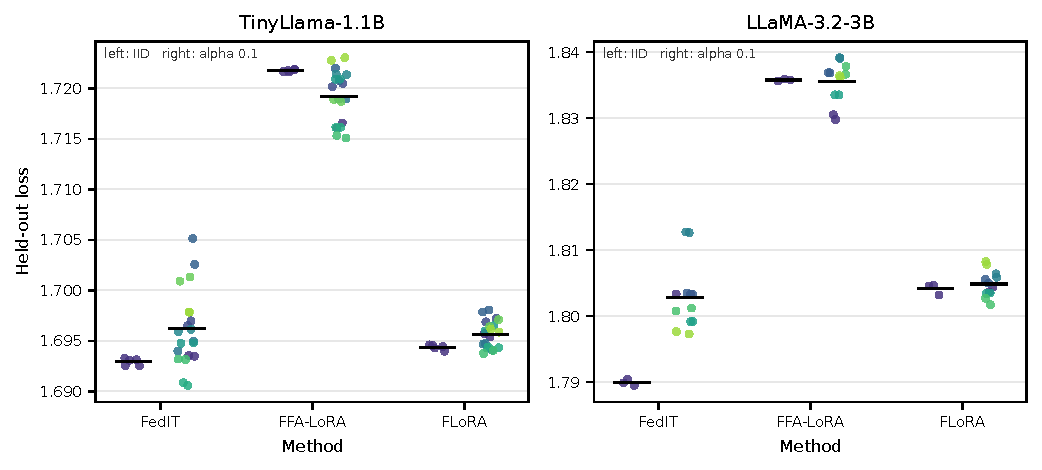
\includegraphics[width=\textwidth]{fig1_heldout_loss.pdf}
\caption{Held-out loss by method and partition at Dirichlet $\alpha{=}0.1$.}
\label{fig:heldout}
\end{figure*}

\begin{figure*}[!t]
\centering
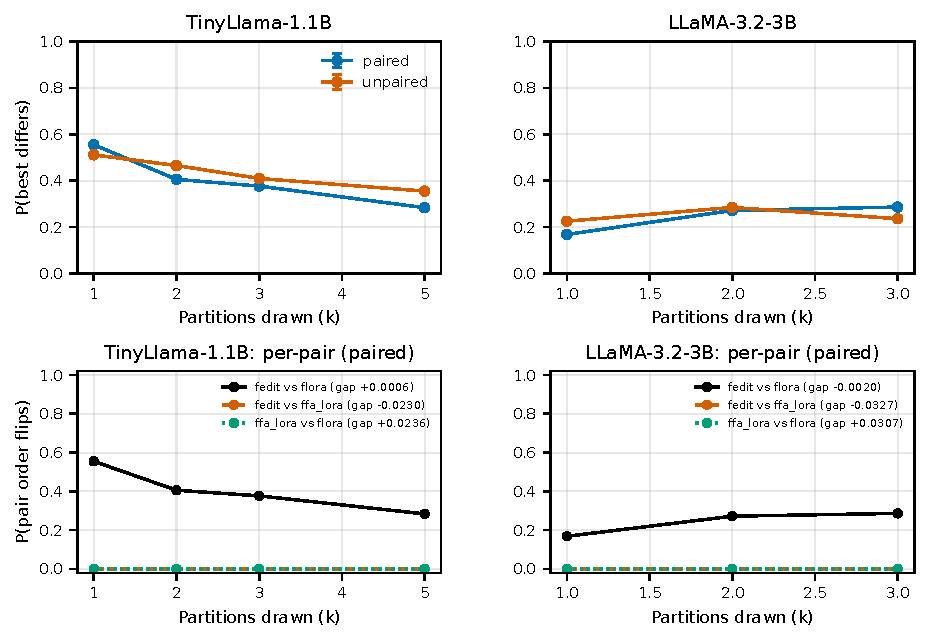
\includegraphics[width=\textwidth]{fig2_rank_flip.pdf}
\caption{Ranking-flip probabilities under paired and unpaired protocols.}
\label{fig:flip}
\end{figure*}

\begin{figure*}[!t]
\centering
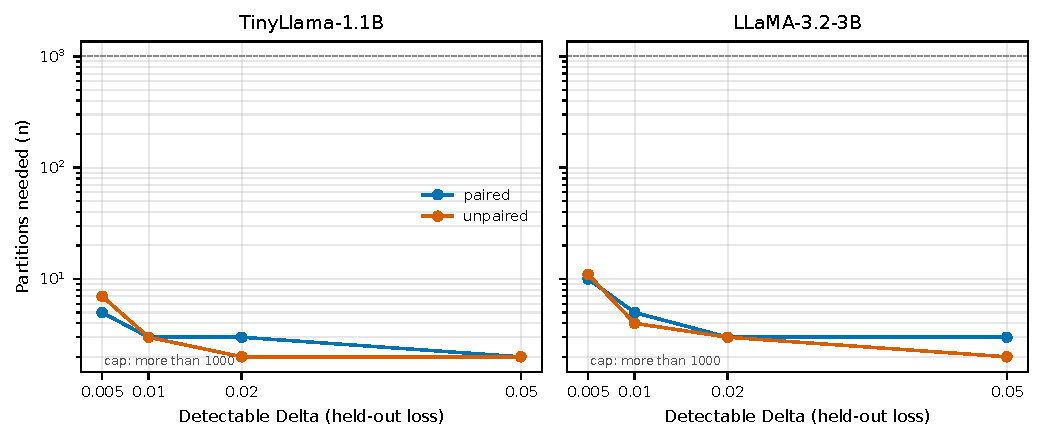
\includegraphics[width=\textwidth]{fig3_draws_needed.pdf}
\caption{Partition draws needed for pre-registered deltas and observed gaps.}
\label{fig:draws}
\end{figure*}

\section{Discussion}
\label{sec:discussion}

\paragraph{What to report.}
A multi-seed mean alone does not answer whether a federated LoRA ranking is stable under the non-IID draw. FFA-LoRA already shows that across-run standard deviations can exceed method gaps~\cite{sun2024ffalora}; our results go one step further by decomposing that variation into a partition component, a partition-by-method interaction, and a residual training-seed component. At Dirichlet $\alpha{=}0.1$, the residual $\hat\sigma^2_E$ is small relative to $\hat\sigma^2_P$ and $\hat\sigma^2_{PM}$ on TinyLlama, so reporting only run seeds understates the uncertainty that matters for ranking. Practical reporting should therefore (i) separate the partition seed from the training seed, (ii) publish the variance shares or at least the paired per-draw SD of method differences, and (iii) state how many partition draws were used. When the observed gap is near that paired SD ($0.00282$ on TinyLlama, $0.00473$ on LLaMA-3.2-3B), a few-draw evaluation is nearly a coin flip; when the gap is about $0.023$ to $0.031$, three paired draws sufficed here.

\paragraph{What pairing fixes, and what it does not.}
Pairing methods on the same partition draws removes the shared partition main effect from the comparison and is the right default for ranking. It does not remove the interaction: methods can still reorder across draws when their responses to a partition differ. That is exactly the FedIT--FLoRA near-tie ($+0.00055$ on TinyLlama, $-0.0020$ on LLaMA), where best-method and full-order flip probabilities coincide because only the top pair moves. Pairing also does not invent power. Detecting a pre-registered $\Delta{=}0.005$ still needs $5$ (TinyLlama) or $10$ (LLaMA) paired draws; the observed near-tie would need $206$ and $46$. Unpaired designs pay a similar or larger sample-size bill. Pairing is therefore a variance-control device, not a substitute for enough independent partitions.

\paragraph{Cross-scale reading.}
On TinyLlama the partition share is substantial ($0.508$). On LLaMA-3.2-3B the interaction dominates ($0.764$) and the partition main-effect CI includes zero, so we do not claim a partition main effect at 3B. Cross-scale CIs on the partition share overlap; the two scales are not distinguishable on that margin. The rise in LLaMA flip probability from $k{=}1$ to $k{=}3$ is a six-partition near-tie artifact, not evidence that more draws hurt. We report the 3B IID floor descriptively only ($2$ degrees of freedom per method) and do not interpret its ratio to $\hat\sigma^2_E$.

\paragraph{Limitations.}
The study uses one dataset (Dolly), one heterogeneity level ($\alpha{=}0.1$), three aggregators, and held-out next-token loss rather than generation benchmarks. LLaMA production holdouts run in float16; the float32 spot-check bound the difference well below the $0.01$ effect scale, but the primary 3B numbers remain float16. Only $6$ partitions support the 3B grid, which widens bootstrap CIs and limits ranking resamples. The MixedLM partition component did not identify, so the mixed-model cross-check is partial and moment estimates are primary. Communication is reported within method only, because FFA-LoRA's implemented payload differs by construction. RQ4 correlations are exploratory and do not replicate at 3B. Adapter weights were not retained for most cells, so the release covers results and metadata rather than full artifacts.

\paragraph{No method recommendation.}
We do not crown FedIT, FFA-LoRA, or FLoRA. The separable FFA-LoRA gaps are large and stable; the FedIT--FLoRA gap is not. The contribution is the measurement design and the conditioning of ranking stability on effect size relative to partition-draw noise.

\section{Conclusion}
\label{sec:conclusion}

At Dirichlet $\alpha{=}0.1$, the partition draw and its interaction with the method are first-order sources of uncertainty in federated LoRA evaluations. On TinyLlama the partition draw alone accounts for about half of held-out-loss variance, with a comparable interaction share; on LLaMA-3.2-3B at ten partition draws the interaction dominates and the partition main-effect interval includes zero after truncation. Extending that 3B grid from six to ten draws reverses the top-two FedIT--FLoRA ordering and multiplies the interaction component by $2.66$, so an evaluation that stopped at six draws would report the wrong ranking and understate interaction variance. Rankings of near-tied methods flip under few draws, while gaps an order of magnitude larger than the per-draw paired SD do not. Detecting the observed FedIT--FLoRA near-tie would require hundreds of paired partitions at 1.1B and more than a thousand at 3B. Evaluations should therefore report how many partition draws were used, pair methods on the same draws, and state the smallest difference the design can detect. We make no method recommendation.


\section*{Declarations}
\paragraph{Data and code availability.}
Code and run artifacts will be released upon acceptance.
\paragraph{Funding.}
None.
\paragraph{Conflicts of interest.}
None.
\paragraph{Generative AI.}
Declaration version to be selected by the author before submission (plan versions a or b).

\balance
\bibliographystyle{IEEEtran}
\bibliography{refs}

\end{document}
